\section{Methods}

\subsection{Overview}
It is assumed that 100\% burnt area will occur under perfect fire conditions -  i.e. full fuel coverage, no moisture, saturated igntions and no agricultural or urban fragmentation. This is analogous to areas in Northern Australia and parts of the sahel which experiance buring each year.
Burnt area is reduced as each limitation becomes sub-optimal, i.e.
    fuel loads become discontinuous  (e.g. desert areas)
    or too moist (e.g. Humid evergreen forests),
    if their is lack of ignition \citep[shown to be an influence inter annual variability in parts Southern Australia][](bradstock2010biogeographic),
    or with increased human influance on the landscape (e.g. cropland or urban areas).
Fraction burnt area ($F$) is therefore the product of the maximum allowed burnt area for each limitation ($F_i$)
\begin{equation}
    F=\Pi_{i} F_i
\end{equation}

$F_i$ is
\begin{equation}
    f(x) = (1 + a * e^{-b \cdot x})
\end{equation}

Our analysis is based on the principle of multiple regressions,
which enables underlying relationships with several predictor
variables to be teased out even in the presence of (moderate)
correlations between the predictors. The finding that a
given predictor has a statistically significant effect on the prediction
means there is a relationship that remains after the
effects of the other predictors have been taken into account.
The form of the burnt-area data – lying between 0 and 1, but
over-dispersed and with many (∼ 90 %) zero values – rules
out the use of ordinary least-squares regression, and calls

Fire increases with increasing fuel load ($F_w$) and igntions ($F_{ig}$), and decreases with moisture ($F_{\omega}$) and anthropagenic supression ($F_s$). Therefore:
\begin{equation}
    \begin{split}
        F_{w} = f(w) \\
        F_{\omega} = 1 - f(\omega) \\
        F_{ig} = f(ig) \\
        F_{s} = 1- f(s)
    \end{split}
\end{equation}

where



\subsubsection{Fuel ($w$)}

\subsubsection{Moisture ($\omega$)}

\paragraph(Live Fuel)
\citep[$\alpha$ ---  measure of availability of water for plants, and a good index for fuel moisture content ---][]{prentice1993simulation}

\paragraph(Dead Fuel)

\subsubsection{Igntions ($ig$)}

\subsubsection{Supression ($s$)}

\subsection{Analysis}

\subsubsection{Limitation}

\begin{equation}
    \bar{l_{i, X}} = \frac{l_{i, X}}{\sum_{j} l_{j, X}}
\end{equation}

\subsubsection{Sensitivity}

\begin{equation}
    \bar{dl_{i, X}} = \frac{dl_{i, X} \cdot \Pi_{j} l_{j, X}}{l_{i, X}}
\end{equation}

where $dl_{i, X}$ is the gradient of $l_{i, X}$ relative to the maximum possible gradient of $l_{i}$, i.e:

\begin{equation}
    dl_{i, X} = \frac{dl_{i, X} / dx}{dl_{i, l = 0.5} / dx}
\end{equation}

where

\begin{equation}
    \frac{dl_{i}}{dx}
\end{equation}

\begin{figure}[!ht]
  \centering
    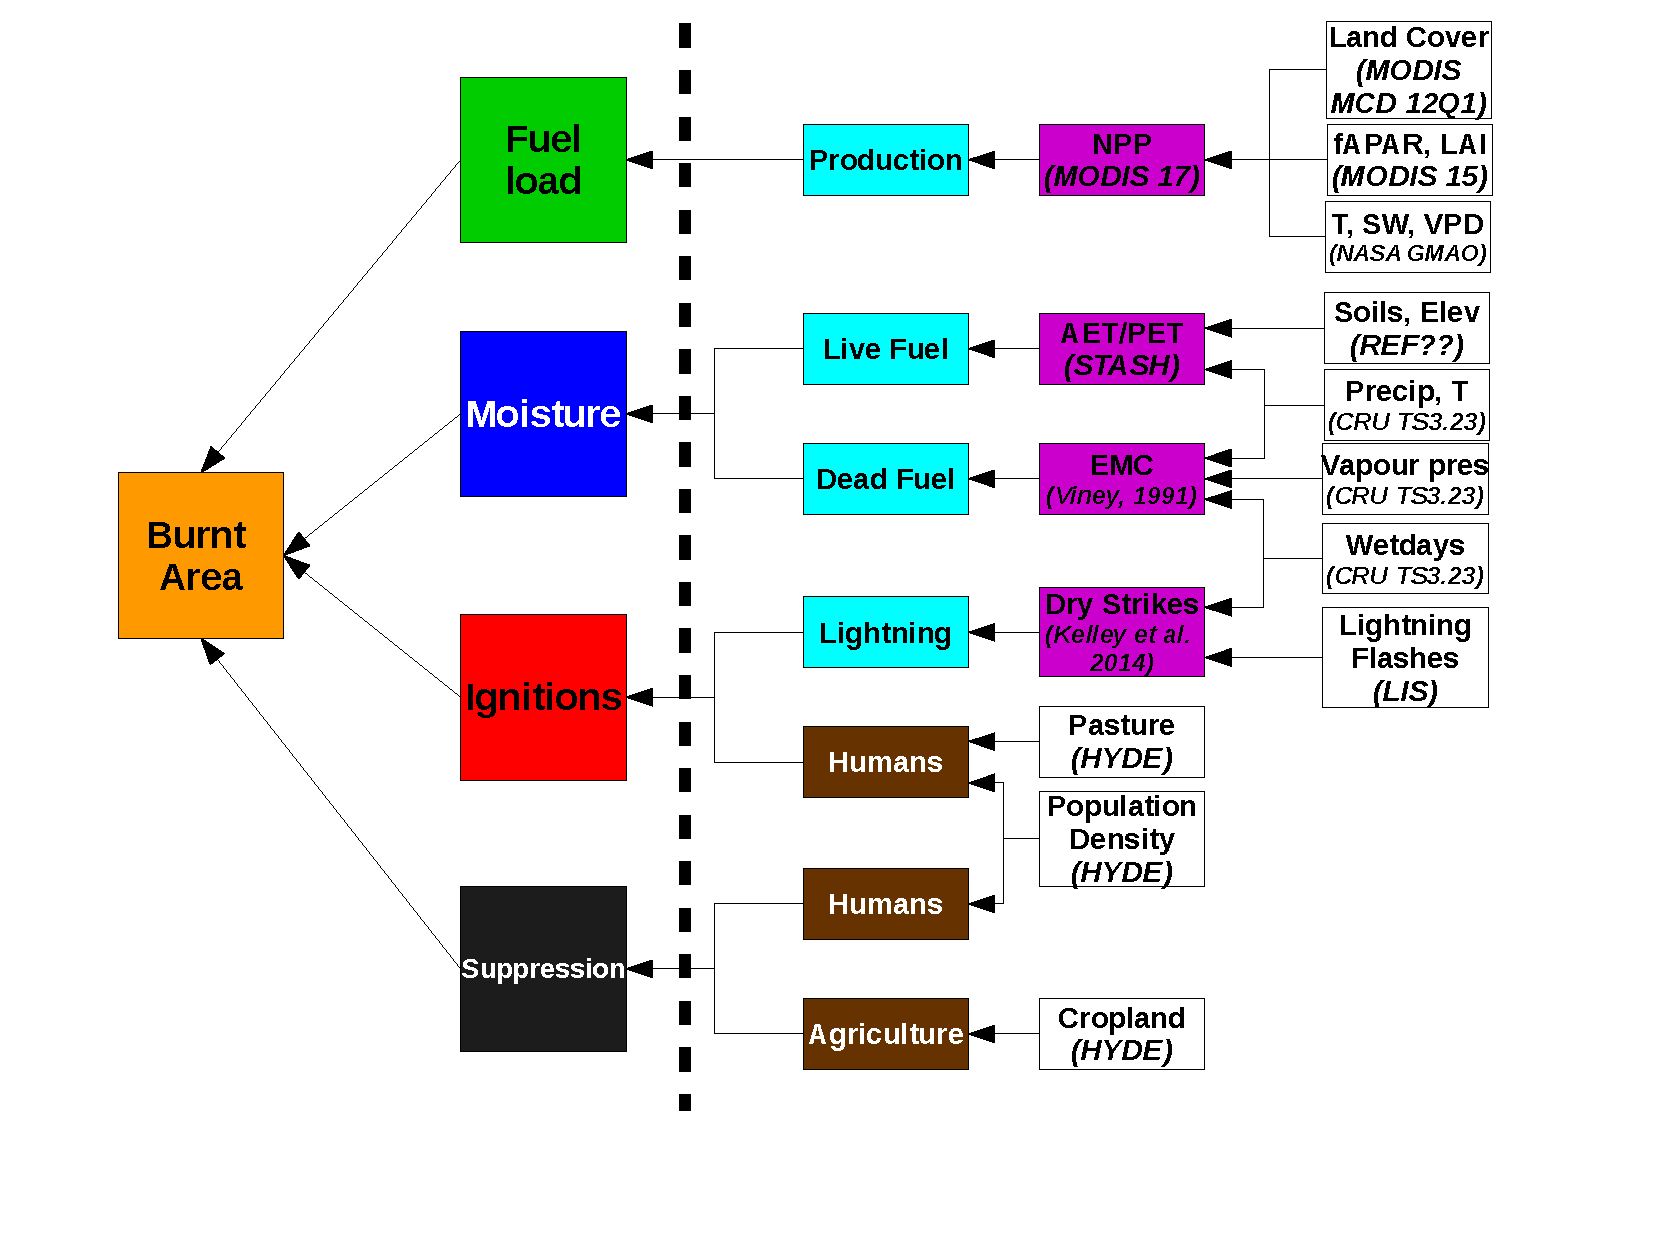
\includegraphics[width=0.67\textwidth]{Model_schematic.pdf}
  \caption{Model description.}
\end{figure}
